\documentclass{beamer}
\mode<presentation>{\usetheme{Madrid}}
\usepackage[utf8]{inputenc}
\usepackage[russian]{babel}
\usepackage{amssymb}
\usepackage{amsmath}
% \usepackage{enumitem}
\usepackage{color}
\usepackage{tabu}
\usepackage{booktabs}
\usepackage{graphicx}
\usepackage{grffile}

\title[Дипломная работа]{Применение задачи классификации для разделения поверхности,
заданной набором космических снимков, на регионы, обладающие почвенной интерпретацией}
\author{Данила Рухович}
\institute[]{Московский государственный университет им. М.В.Ломоносова \\
Механико-математический факультет}
\date{26 мая, 2017}

\begin{document}

\begin{frame}
\titlepage
\end{frame}

\begin{frame}
\frametitle{План}
\begin{enumerate}
    \item {\color{blue}Постановка задачи}
        \begin{itemize}
            \item Задача обучения по прецендентам
            \item Задача классификации типов почв по комическим снимкам
            \item Актуальность
        \end{itemize}
    \item Предлагаемое решение
    \begin{itemize}
        \item Классификационные модели
        \item Данные для экспериментов
        \item Модель линии почвы
        \item Предобработка снимков
        \item Признаковое описание объектов
    \end{itemize}
    \item Эксперименты
    \begin{itemize}
        \item Классификация по данным почвенных разрезов
        \item Классификация по данным почвенной карты
    \end{itemize}
    \item Заключение
\end{enumerate}
\end{frame}

\begin{frame}
\frametitle{Задача обучения по прецендентам}
\begin{block}{Пусть:}
$\mathcal{X}$ - множество объектов \\
$\mathcal{Y}$ - множество ответов \\
$\hat{y}:\mathcal{X} \to \mathcal{Y}$ - неизвестная зависимость \\
\end{block}
\begin{block}{Дано:}
$X = \{x_i\}_{i=1}^m \in \mathcal{X}$ - обучающая выборка \\ 
$Y = \{y_i\}_{i=1}^m$ - известные ответы \\
$\{f_j\}_{j=1}^n$, $f_j:\mathcal{X} \to \mathbb{R}$ - признаковые описания
\end{block}
\begin{block}{Найти:}
$a:X \to \mathcal{Y}$ - решающую функцию, приближающую $\hat{y}$ на $\mathcal{X}$
\end{block}
\begin{block}{Частный случай - задача классификации}
$\mathcal{Y}=\{1, ..., M\}$ - конечное множество меток непересекающихся классов
\end{block}
\end{frame}

\begin{frame}
\frametitle{Постановка задачи классификации типов почв по космическим снимкам}
\begin{itemize}
\item \textbf{Множество объектов} - точки на поверхности Замли
\item \textbf{Множество ответов} - типы почв, встречающиеся на исследуемой территории
\item \textbf{Признаковые описания} - конструируются из набора космических снимков территории
\end{itemize}
\end{frame}

\begin{frame}
\frametitle{Актуальность}
\footnotesize{
\begin{thebibliography}{9}
\bibitem[]{} Nanni M.R., Dematte J.A. et al
\newblock Soil surface spectral data from Landsat imagery for soil class discrimination
\newblock \emph{Acta Scientiarum Agronomy} (2012) 34
\bibitem[]{} Украинский П.А., Землякова А.В.
\newblock Определение параметров почвенной линии
для автоматического распознавания открытой поверхности почвы на космических снимках
\newblock \emph{Международный журнал прикладных и фундаментальных исследований} (2014) 9
\bibitem[]{} Черный С.Г., Абрамов Д.А.
\newblock Определение параметров линии почв черноземов
правобережной Украины с помощью спектральных спутниковых снимков Ландсат-7
\newblock \emph{Gruntoznavstvo} (2013) 14
\end{thebibliography}}
\end{frame}

\iffalse
\begin{frame}
\frametitle{Новизна}
\footnotesize{
\begin{thebibliography}{9}
\bibitem[]{} Rukhovich D.I., Rukhovich A.D., Rukhovich D.D. et al
\newblock The informativeness of coefficients a and b of the
soil line for the analysis of remote sensing materials
\newblock \emph{Eurasian Soil Science} (2016) 49
\bibitem[]{} Rukhovich D.I., Rukhovich A.D., Rukhovich D.D. et al
\newblock The Application of the Piecewise Linear Approximation
to the Spectral Neighborhood of Soil Line for the Analysis
of the Quality of Normalization of Remote Sensing Materials
\newblock \emph{Eurasian Soil Science} (2017) 50
\bibitem[]{} Rukhovich D.I., Rukhovich A.D., Rukhovich D.D. et al
\newblock  Maps of Averaged Spectral Deviations from Soil Lines
and Their Comparison with Traditional Soil Maps
\newblock \emph{Eurasian Soil Science} (2016) 49
\end{thebibliography}}
\end{frame}
\fi

\begin{frame}
\frametitle{План}
\begin{enumerate}
    \item Постановка задачи
        \begin{itemize}
            \item Задача обучения по прецендентам
            \item Задача классификации типов почв по комическим снимкам
            \item Актуальность
        \end{itemize}
    \item {\color{blue} Предлагаемое решение}
    \begin{itemize}
        \item Классификационные модели
        \item Данные для экспериментов
        \item Модель линии почвы
        \item Предобработка снимков
        \item Признаковое описание объектов
    \end{itemize}
    \item Эксперименты
    \begin{itemize}
        \item Классификация по данным почвенных разрезов
        \item Классификация по данным почвенной карты
    \end{itemize}
    \item Заключение
\end{enumerate}
\end{frame}

\begin{frame}
\frametitle{Использумые методы}
\begin{block}{Классификаторы}
\begin{itemize}
    \item Метод ближаших соседей (k Nearest Beaighbors)
    \item Случайный лес (Random Forest)
    \item Метод опорных векторов (SVM)
    \item Байесовский классификатор (Naive Bayes classifier)
    \item Логистическая регрессия (Logistic Regression)
    \item Градиентный бустинг над решающими деревьями (Xgboost)
\end{itemize}
\end{block}
\begin{block}{Оценка качества}
Скользящий контроль по $q$ блокам (q-fold Cross Validation)
\end{block}
\begin{block}{Функционал качества}
Точность (accuracy)
\end{block}
\end{frame}

\begin{frame}
\frametitle{Данные для экспериментов}
\begin{itemize}
    \item 35 фрагментов спутников Landsat
    \item информация о 1761 почвенном разрезе
    \item информация о 2503407 точках почвенной карты
\end{itemize}
\end{frame}

\begin{frame}
\frametitle{Данные для экспериментов}
\begin{block}{Список используемых снимков}
\begin{table}[H]
\centering
\begin{tabu}{|l|l|l|}
    \hline
    \multicolumn{1}{|c|}{Номер} & \multicolumn{1}{c|}{Спутник} & \multicolumn{1}{c|}{Дата} \\
    \tabucline[1.5pt]{-} 
           1 & Landsat 5 & 16.05.1985 \\
    \hline 2 & Landsat 5 & 04.08.1985 \\
    \hline ... & ... & ... \\
    \hline 16& Landsat 7 & 06.10.1999 \\
    \hline 17& Landsat 7 & 17.05.2000 \\
    \hline ... & ... & ... \\
    \hline 34& Landsat 8 & 16.03.2015 \\
    \hline 35& Landsat 8 & 06.07.2015 \\
    \hline
\end{tabu}
\end{table}
\end{block}
\end{frame}

\begin{frame}
\frametitle{Данные для экспериментов}
\begin{block}{Список каналов Landsat 8}
\begin{table}[H]
\centering
\begin{tabu}{|l|m{5cm}|l|}
    \hline
    \multicolumn{1}{|c|}{Номер} & \multicolumn{1}{c|}{Название} 
    & \multicolumn{1}{c|}{Разрешение} \\
    \tabucline[1.5pt]{-}
           1 & Побережья и аэрозоли (New Deep Blue) & 30 м \\
    \hline 2 & Синий (Blue) & 30 м \\
    \hline 3 & Зеленый (Green) & 30 м \\
    \hline 4 & Красный (Red) & 30 м \\
    \hline 5 & Ближний ИК (NIR) & 30 м \\
    \hline 6 & Ближний ИК (SWIR2) & 30 м \\
    \hline 7 & Ближний ИК (SWIR3) & 30 м \\
    \hline 8 & Панхроматический (PAN) & 15 м \\
    \hline 9 & Перистые облака (SWIR) & 30 м \\
    \hline 10& Дальний ИК (TIR1) & 100 м \\
    \hline 11& Дальний ИК (TIR2) & 100 м \\
    \hline
\end{tabu}
\end{table}
\end{block}
\end{frame}

\begin{frame}
\frametitle{Данные для экспериментов}
\begin{figure}[H]
\centering
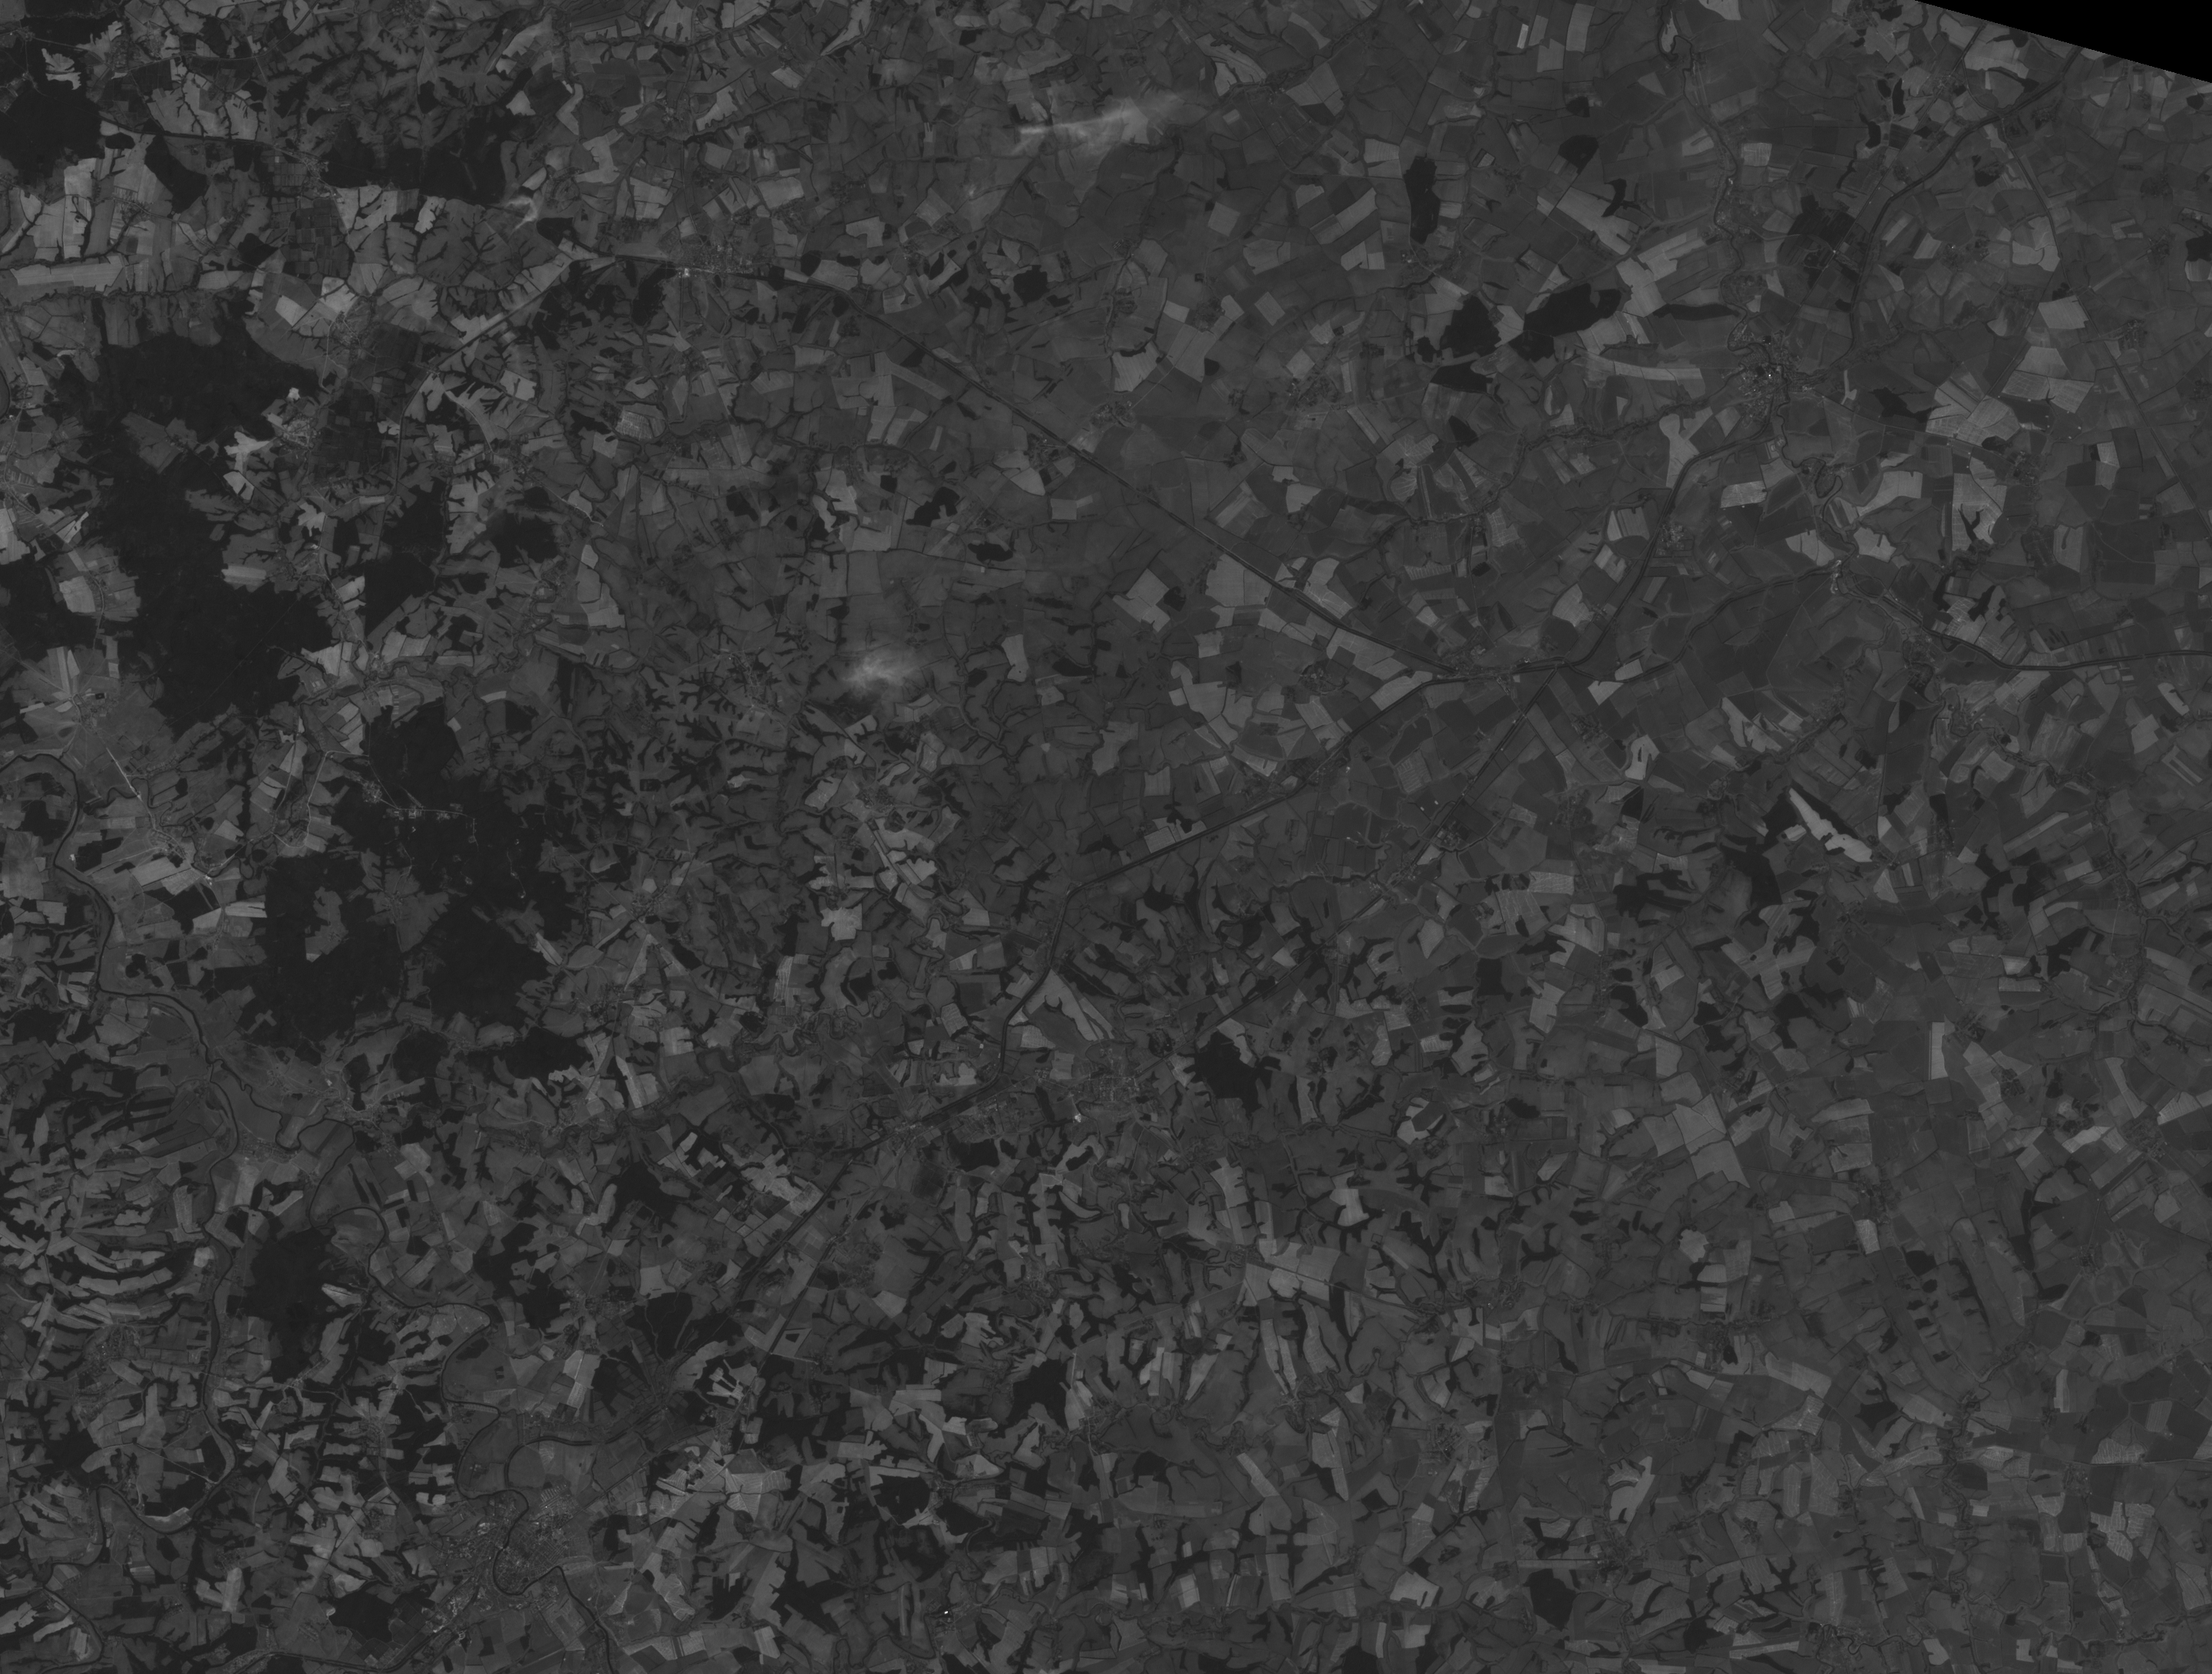
\includegraphics[width=0.8\linewidth]{imgs/landsat_example.png}
\end{figure}
\end{frame}

\begin{frame}
\frametitle{Модель линии почвы}
\begin{figure}[H]
\centering
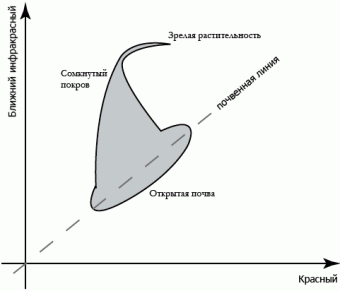
\includegraphics[width=0.7\linewidth]{imgs/soil_line_model.png}
\end{figure}
\end{frame}

\begin{frame}
\frametitle{Модель линии почвы}
\begin{figure}[H]
\centering
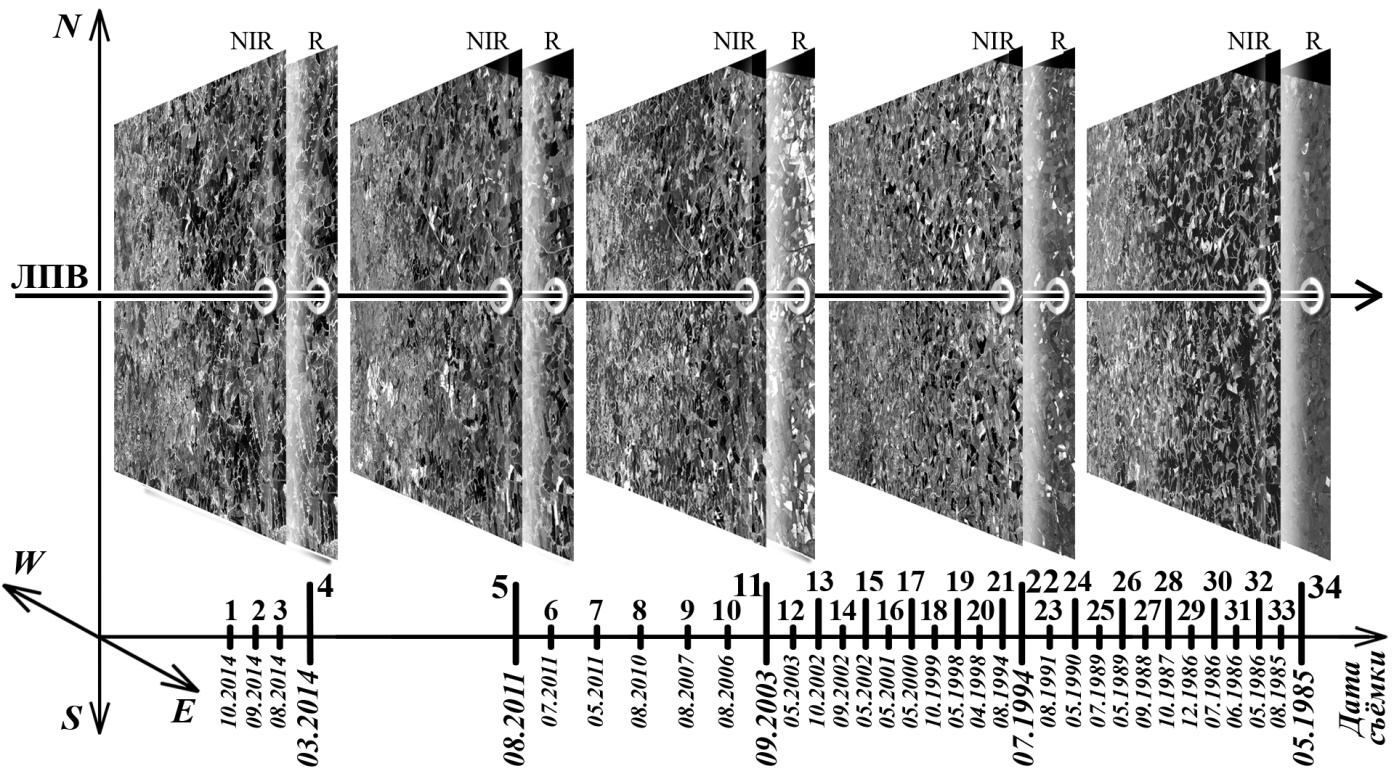
\includegraphics[width=0.7\linewidth]{imgs/soil_line_time.png}
\end{figure}
\end{frame}

\begin{frame}
\frametitle{Предобработка снимков}
\begin{enumerate}
    \item Фильтрация снимков
    \item Нормализация снимков
    \begin{itemize}
        \item Классическая (mean+std)
        \item Атмосферная коррекция (rad+refl)
        \item Исходные данные (none)
    \end{itemize}
    \item Усреднение снимков
\end{enumerate}
\end{frame}

\begin{frame}
\frametitle{Признаковое описание объектов}
\begin{enumerate}
\item Среднее, дисперсия, минимум, максимум:
    \begin{itemize}
        \item Красный (red)
        \item Ближний инфракрасный (nir)
        \item Зеленый (green)
        \item Синий (blue)
    \end{itemize}
\item Коэффициент наклона линии почвы временной
\item Процент неотфильтрованных значений
\end{enumerate}
\end{frame}

\begin{frame}
\frametitle{План}
\begin{enumerate}
    \item Постановка задачи
        \begin{itemize}
            \item Задача обучения по прецендентам
            \item Задача классификации типов почв по комическим снимкам
            \item Актуальность
        \end{itemize}
    \item Предлагаемое решение
    \begin{itemize}
        \item Классификационные модели
        \item Данные для экспериментов
        \item Модель линии почвы
        \item Предобработка снимков
        \item Признаковое описание объектов
    \end{itemize}
    \item {\color{blue} Эксперименты}
    \begin{itemize}
        \item Классификация по данным почвенных разрезов
        \item Классификация по данным почвенной карты
    \end{itemize}
    \item Заключение
\end{enumerate}
\end{frame}

\begin{frame}
\frametitle{Классификация по данным почвенных разрезов}
\begin{figure}[H]
\centering
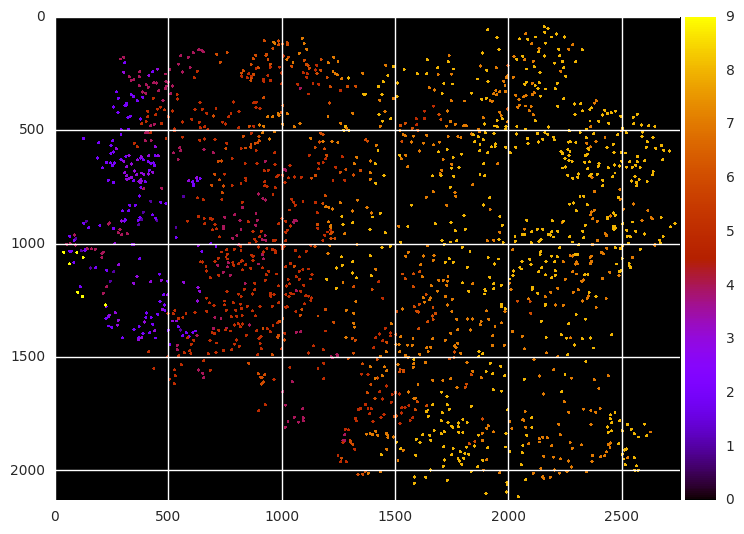
\includegraphics[width=0.8\linewidth]{imgs/cuts.png}
\end{figure}
\end{frame}

\begin{frame}
\frametitle{Классификация по данным почвенных разрезов}
\begin{figure}[H]
\centering
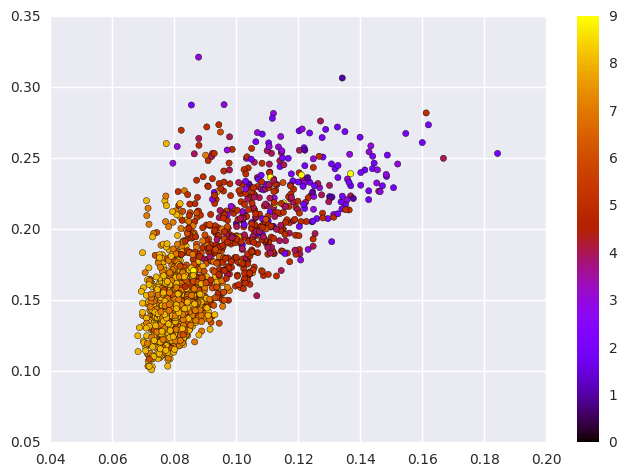
\includegraphics[width=0.8\linewidth]{imgs/projection.png}
\end{figure}
\end{frame}

\begin{frame}
\frametitle{Классификация по данным почвенных разрезов}
\begin{table}[H]
\centering
\begin{tabu}{|l|l|l|}
    \hline
    \multicolumn{1}{|c|}{Классификатор} & \multicolumn{1}{c|}{Точность, 9 классов} 
    & \multicolumn{1}{c|}{Точность, 3 класса} \\
    \tabucline[1.5pt]{-} 
           kNN & 54.9\% & 88.5\% \\
    \hline Random Forest & 60.5\% & 91.2\% \\ 
    \hline SVM & 59.1\% & 90.2\% \\
    \hline Bayesian & 54.1\% & 85.9\% \\
    \hline Log Regression & 53.2\% & 90.0\% \\
    \hline Xgboost & 59.7\% & 91.0\% \\
    \hline
\end{tabu}
\end{table}
\end{frame}

\begin{frame}
\frametitle{Классификация по данным почвенных разрезов}
\begin{table}[H]
\centering
\begin{tabu}{|l|l|l|}
    \hline
    \multicolumn{1}{|c|}{Нормализация} & \multicolumn{1}{c|}{Точность, 9 классов} & 
    \multicolumn{1}{c|}{Точность, 3 класса} \\
    \tabucline[1.5pt]{-}
           mean+std & 60.5\% & 90.6\% \\
    \hline none & 59.5\% & 89.4\% \\
    \hline rad+refl & 63.1\% & 91.2\% \\
    \hline
\end{tabu}
\end{table}
\end{frame}

\begin{frame}
\frametitle{Классификация по данным почвенных разрезов}
\begin{figure}[H]
\centering
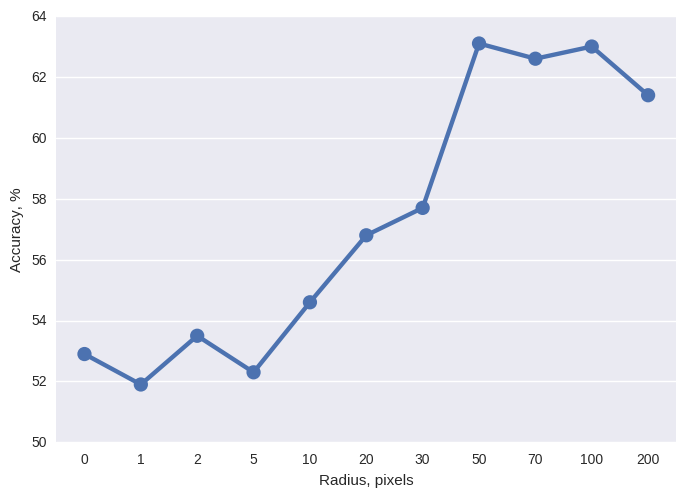
\includegraphics[width=0.8\linewidth]{imgs/cuts_radius.png}
\end{figure}
\end{frame}

\begin{frame}
\frametitle{Классификация по данным почвенных разрезов}
\begin{figure}[H]
\centering
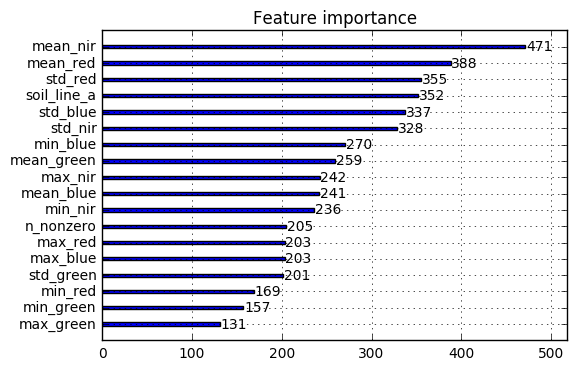
\includegraphics[width=0.8\linewidth]{imgs/cuts_importance.png}
\end{figure}
\end{frame}

\begin{frame}
\frametitle{Классификация по данным почвенной карты}
\begin{figure}[H]
\centering
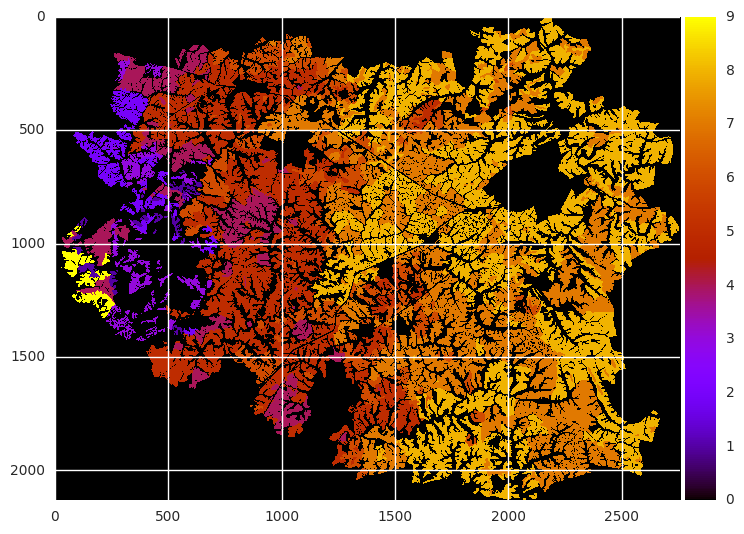
\includegraphics[width=0.8\linewidth]{imgs/map.png}
\end{figure}
\end{frame}

\begin{frame}
\frametitle{Классификация по данным почвенной карты}
\begin{table}[H]
\centering
\begin{tabu}{|l|l|l|}
    \hline
    \multicolumn{1}{|c|}{Классификатор} & \multicolumn{1}{c|}{Точность, 9 классов} 
    & \multicolumn{1}{c|}{Точность, 3 класса} \\
    \tabucline[1.5pt]{-} 
           kNN & 72.9\% & 94.6\% \\
    \hline Random Forest & 78.9\% & 95.2\% \\ 
    \hline SVM & 70.2\% & 95.6\%\\
    \hline Bayesian & 52.5\% & 89.1\% \\
    \hline Log Regression & 56.8\% & 90.1\% \\
    \hline Xgboost & 80.1\% & 95.7\% \\
    \hline
\end{tabu}
\end{table}
\end{frame}

\begin{frame}
\frametitle{Классификация по данным почвенной карты}
\begin{table}[H]
\centering
\begin{tabu}{|l|l|l|}
    \hline
    \multicolumn{1}{|c|}{Нормализация} & \multicolumn{1}{c|}{Точность, 9 классов}
    & \multicolumn{1}{c|}{Точность, 3 класса} \\
    \tabucline[1.5pt]{-}
           mean+std & 80.1\% & 95.3\% \\
    \hline none & 78.9\% & 95.1\% \\
    \hline rad+refl & 81.2\% & 95.7\%\\
    \hline
\end{tabu}
\end{table}
\end{frame}

\begin{frame}
\frametitle{Классификация по данным почвенной карты}
\begin{figure}[H]
\centering
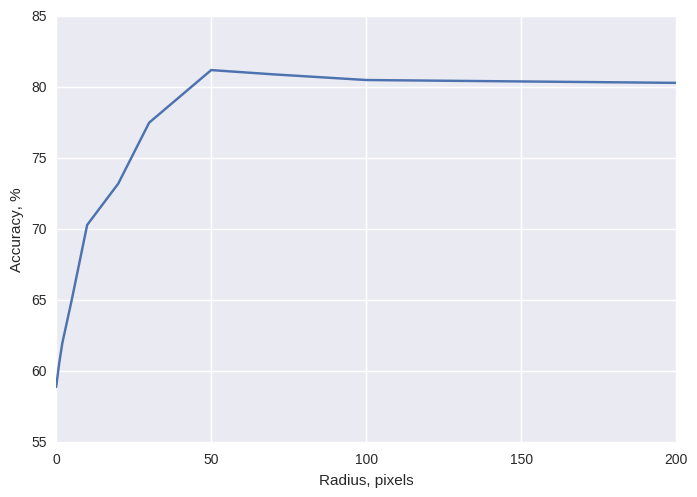
\includegraphics[width=0.8\linewidth]{imgs/map_radius.png}
\end{figure}
\end{frame}

\begin{frame}
\frametitle{Классификация по данным почвенной карты}
\begin{figure}[H]
\centering
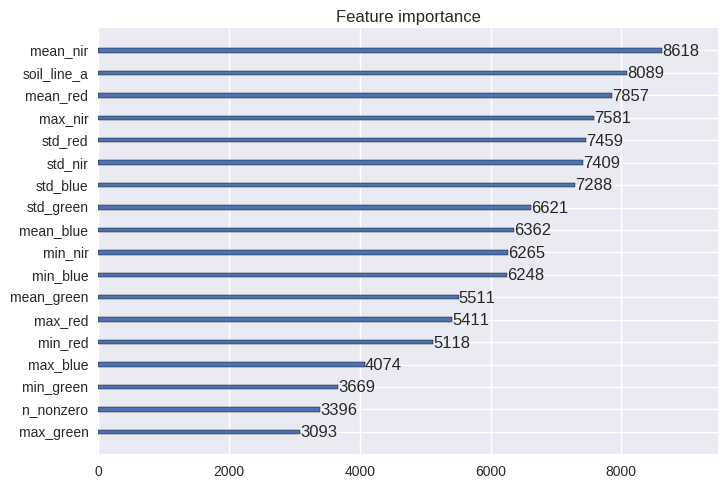
\includegraphics[width=0.8\linewidth]{imgs/map_importance.png}
\end{figure}
\end{frame}

\begin{frame}
\frametitle{Классификация по данным почвенной карты}
\begin{figure}[H]
\centering
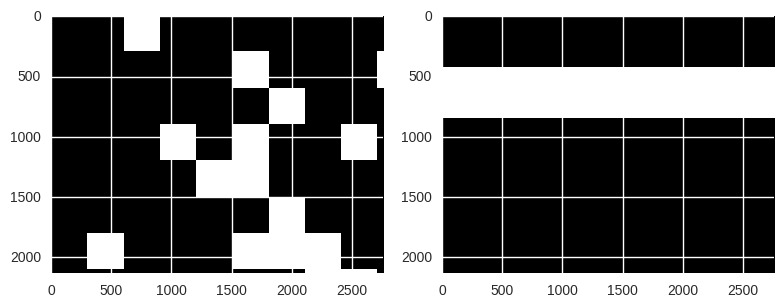
\includegraphics[width=0.8\linewidth]{imgs/validation_masks.png}
\end{figure}
\end{frame}

\begin{frame}
\frametitle{Классификация по данным почвенной карты}
\begin{figure}[H]
\centering
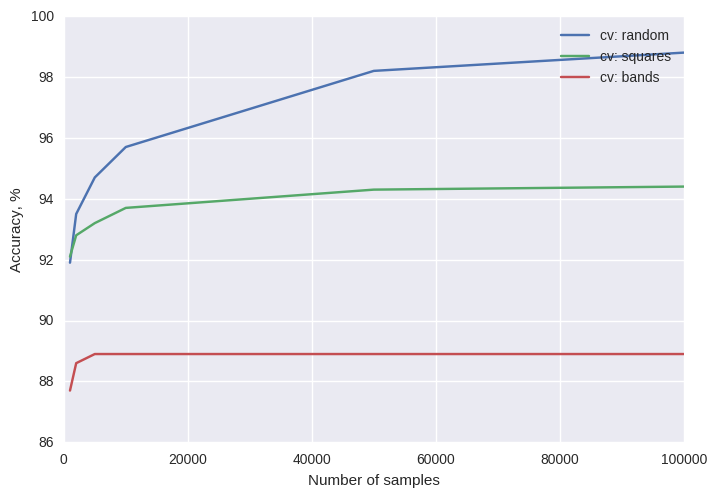
\includegraphics[width=0.8\linewidth]{imgs/map_validations_3_classes.png}
\end{figure}
\end{frame}

\begin{frame}
\frametitle{Классификация по данным почвенной карты}
\begin{figure}[H]
\centering
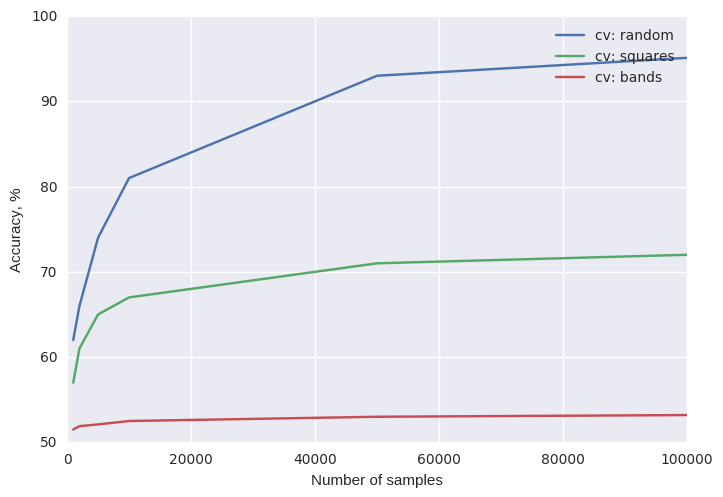
\includegraphics[width=0.8\linewidth]{imgs/map_validations_9_classes.png}
\end{figure}
\end{frame}

\begin{frame}
\frametitle{План}
\begin{enumerate}
    \item Постановка задачи
        \begin{itemize}
            \item Задача обучения по прецендентам
            \item Задача классификации типов почв по комическим снимкам
            \item Актуальность
        \end{itemize}
    \item Предлагаемое решение
    \begin{itemize}
        \item Классификационные модели
        \item Данные для экспериментов
        \item Модель линии почвы
        \item Предобработка снимков
        \item Признаковое описание объектов
    \end{itemize}
    \item Эксперименты
    \begin{itemize}
        \item Классификация по данным почвенных разрезов
        \item Классификация по данным почвенной карты
    \end{itemize}
    \item {\color{blue} Заключение}
\end{enumerate}
\end{frame}

\begin{frame}
\frametitle{Заключение}
\begin{block}{Исследованы:}
\begin{enumerate}
    \item Применимость стандартных алгоритмов задачи классификации
    \item Целесообразность использования набора разновременных снимков 
    \item Информативность коэффициентов линии почвы временной
    \item Влияние типа нормализации и радиуса усреднения снимков 
\end{enumerate}
\end{block}
\begin{block}{Достигнуты точности:}
\begin{enumerate}
    \item При классификации по почвенным разрезам:
    \begin{itemize}
        \item 3 класса: 91\%
        \item 9 классов: 63\%
    \end{itemize}
    \item При классификации по почвенной карте (для 3 типов валидации):
    \begin{itemize}
        \item 3 класса: 98\%, 94\%, 89\%
        \item 9 классов: 94\%, 71\%, 50\%
    \end{itemize}
\end{enumerate}
\end{block}
\end{frame}

\end{document}
